% Este archivo es parte de la memoria del proyecto fin de carrera
% de Manuel López Urbina. Protegida bajo la licencia GFDL.
% Para más información, la licencia completa viene incluida en el
% fichero fdl-1.3.tex

% Copyright (C) 2018 Manuel López Urbina

\newpage

\begin{appendix}
\backmatter

\chapter{Anexos}
\label{appendix:anexos}

Anexos con los diferentes elementos software utilizados en el proyecto junto con las instrucciones para la instalación.\\

\section{Arduino, entorno de desarrollo}

El entorno de desarrollo (IDE) ofrecido por Arduino es el que nos permite escribir el programa y cargarlo en la placa, siendo posible su carga de dos maneras:

\begin{figure}[H]
  \begin{center}
    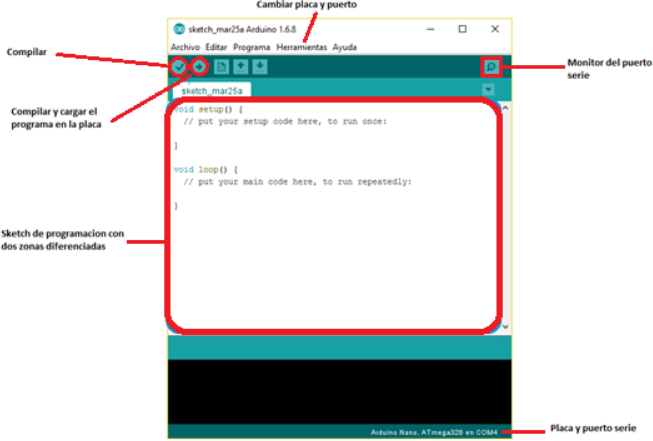
\includegraphics[scale=0.3]{imagenes/entorno_desarrollo_arduino.png}
  \end{center}
  \label{fig:logo}
 \caption{Entorno de desarrollo de Arduino.}
\end{figure}

El software de desarrollo de Arduino es publicado bajo una licencia libre y gratuita, la cual se puede descargar desde la página oficial
incluyendo los drivers necesarios para cualquier placa Arduino, así como las librerías necesarias para su programación.

\begin{enumerate}
 \item Si deseamos trabajar sin conexión, debemos descargar e instalar la versión más reciente
de Arduino desde la página Arduino\footnote{\url{https://www.arduino.cc/en/Main/Software}}.
\item Si tenemos una conexión de internet fiable, podemos usar el IDE online ya que siempre
tendremos la última versión más actualizada del IDE, además de tener disponible
nuestros códigos en la nube y poder acceder a su contenido a través de cualquier
dispositivo y todo eso sin la necesidad de instalar actualizaciones nuevas. A
continuación, Link para acceder al IDE online \footnote{ \url{https://create.arduino.cc/}}.
\end{enumerate}

\subsection{Descarga e instalación}

Para descargar el IDE en nuestro sistema operático solo tendremos que seguir unos sencillos
pasos:

\begin{enumerate}
 \item Descargar el programa gratuito Arduino IDE haciendo clic en el enlace anterior o dirigir a
la web después Software.


\begin{figure}[H]
  \begin{center}
    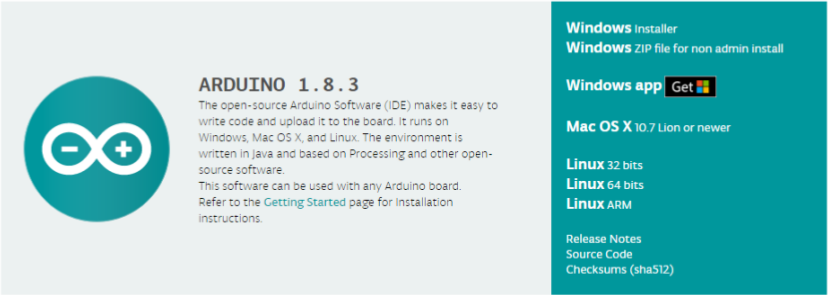
\includegraphics[scale=0.3]{imagenes/descarga_arduino.png}
  \end{center}
  \label{fig:descarga_arduino}
 \caption{Enlace para la descarga del software de Arduino.}
 \end{figure}
 
\item A continuación, podemos elegir entre Arduino web, pudiendo trabajar sin necesidad de descargar ningún software u
optar por descargar Arduino IDE. Para su instalación solo tenemos que elegir nuestro sistema operativo y
seguir las instrucciones de instalación.

\begin{figure}[H]
  \begin{center}
    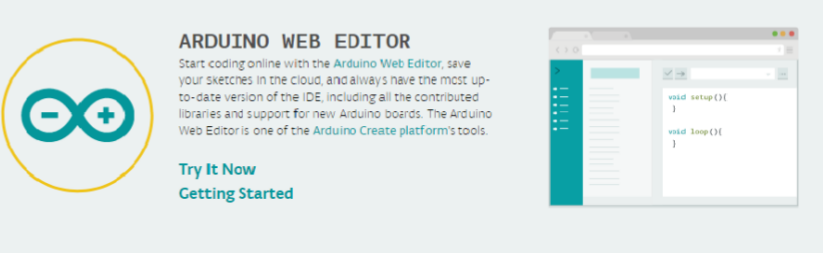
\includegraphics[scale=0.3]{imagenes/arduino_web_ide.png}
  \end{center}
  \label{fig:descarga_arduino}
 \caption{Enlace de acceso al IDE de Arduino en su versión web.}
 \end{figure}

\end{enumerate}

\section{Fritzing}

Es una iniciativa de hardware de código abierto que hace que la electrónica sea accesible como
material creativo para todos, que nos permita hacer diagramas, circuitos electrónicos y
montajes, también sirve para hacer circuitos impresos PCB. También nos permite documentar nuestros prototipos y compartirlos con otros.

\subsection{Descarga e instalación}

Para descargar Fritzing, accesible en el enlace inferior, donde tan solo debemos seleccionar nuestro sistema operativo y hacer clcick en Download. \\

\url{http://fritzing.org/download/?donation=0}

\begin{figure}[H]
  \begin{center}
    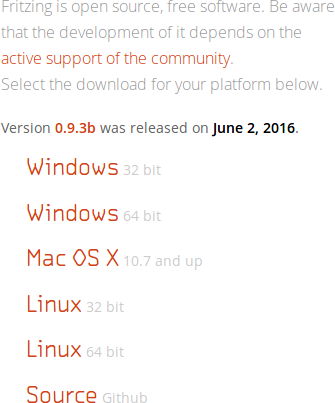
\includegraphics[scale=0.5]{imagenes/fritzing_download.png}
  \end{center}
  \label{fig:descarga_arduino}
 \caption{Sistemas operativos disponibles para Fritzing.}
 \end{figure}

Para su instalación en versión linux debemos seguir los siguientes pasos:

Nos dirigimos al directorio donde hemos realizado la descarga:

\begin{lstlisting}[language=bash]
cd ~/Downloads
\end{lstlisting}

Posteriormente descomprimimos el archivo con el siguiente comando:

\begin{lstlisting}[language=bash]
unzip -xzf fritzing-0.9.3b.linux.AMD64.tar.bz2
\end{lstlisting}


Nos posicionamos en el directorio de trabajo de Fritzing:

\begin{lstlisting}[language=bash]
cd /home/wali/Downloads/fritzing-0.9.3b.linux.AMD64/
\end{lstlisting}


Ejecutamos Fritzing:


\begin{lstlisting}[language=bash]
./Fritzing
\end{lstlisting}

o:

\begin{lstlisting}[language=bash]
sh Fritzing
\end{lstlisting}


\section{Instalación de Node.js}

Instalación de los prerrequisitos:\\

\begin{lstlisting}[language=bash]
sudo apt-get install python-software-properties python g++ make
\end{lstlisting}


Si está utilizando Ubuntu 16.04, necesitará hacer los siguiente:\\

\begin{lstlisting}[language=bash]
sudo apt-get install software-properties-common
\end{lstlisting}


Añadimos el repositorio:\\

\begin{lstlisting}[language=bash]
sudo add-apt-repository ppa:chris-lea/node.js
\end{lstlisting}

Actualizamos la lista de paquetes:\\

\begin{lstlisting}[language=bash]
sudo apt-get update
\end{lstlisting}

Instalación de  Node.js:\\

\begin{lstlisting}[language=bash]
sudo apt-get install nodejs
\end{lstlisting}

\section{Instalación del control de versiones Git}

Para seguir esta guía es necesario disponer de una máquina con Ubuntu 14.04.\\

La forma más sencilla de tener Git instalado y configurado para su utilización es mediante el uso de los repositorios predeterminados de Ubuntu. 
Este es el método más rápido, pero, por contra puede ser que la versión disponible no sea la más reciente. 
Si necesita la última versión, deberá seguir los pasos para compilar Git desde el origen.\\

Si no necesitamos disponer de la última versión podemos instalarlo desde el repositorio de Ubuntu. Para ello introducimos los siguientes comandos en una terminal:\\

\begin{lstlisting}[language=bash]
sudo apt-get update
sudo apt-get install git
\end{lstlisting}

Esto descargará e instalará Git en el sistema. A continuación se describe los pasos para su configuración.

\subsection{Configuración}

Una vez que disponemos de Git instalado, necesitamos realizar una serie de pasos para añadir nuestros datos de acceso de nuestro repositorio.\\

La forma más sencilla de hacerlo es a través del comando \emph{git config} proporcionando nuestro nombre y dirección de correo electrónico. Esto es debido a que Git incorpora esta información en cada commit
que hacemos. Por ejemplo, si nuestro nombre es \emph{RobotUI} y nuestro email \emph{email@robotui.com}, los comandos de configuración serían los siguientes:\\

\begin{lstlisting}[language=bash]
 git config --global user.name "RobotUI"
 git config --global user.email "email@robotui.com"
\end{lstlisting}

Finalmente podemos comprobar todos los valores de configuración establecidos escribiendo:\\

\begin{lstlisting}[language=bash]
git config --list
\end{lstlisting}

Existen muchas más opciones configurables pero estos son los dos esenciales necesarios.\\


\section{Datasheets}

\end{appendix}





